\documentclass[10pt,a4paper]{article}
\usepackage[utf8]{inputenc}
\usepackage[english]{babel}
\usepackage{amsmath}
\usepackage{amsfonts}
\usepackage{amssymb}
\usepackage{graphicx}
\usepackage{float}

\usepackage{helvet}
\usepackage{footnote}
\usepackage{listings}
\usepackage{color}
\definecolor{mygray}{rgb}{0.5,0.5,0.5}
\definecolor{mygreen}{rgb}{0,0.3,0}
\lstset{language=Matlab,
	breaklines=true,
	frame=single,
	basicstyle=\footnotesize,  
	flexiblecolumns=true,
	keywordstyle=\color{blue},
	commentstyle=\color{mygreen},
	captionpos=b,   
}
\renewcommand\familydefault{\sfdefault}
\usepackage[left=2.5cm,right=2.5cm,top=2.5cm,bottom=2.5cm]{geometry}
\title{Athens Course \\Genetic Algorithms: Report}
\author{Stefan Pante\\ KULeuven University}
\begin{document}
\begin{titlepage}
\maketitle
\tableofcontents
\end{titlepage}
\section{Introduction}
\noindent \textbf{Problem:}
A hypothetical town has buildings at 50 locations on a grid. The coordinates for these locations are given by $(i,j)$ where $i = 1,2,\cdots, 10$ and $j = 1,2, \cdots, 5$. A river runs through the town on $j = 3.5$. A fire unit needs to be places somewhere inside the range of the buildings. The average response time should be optimal for all the buildings in the town. A location for the building needs to be calculated. A schematic diagram can be seen in Figure \ref{fig:diagram}.



\begin{figure}[H]
\centering
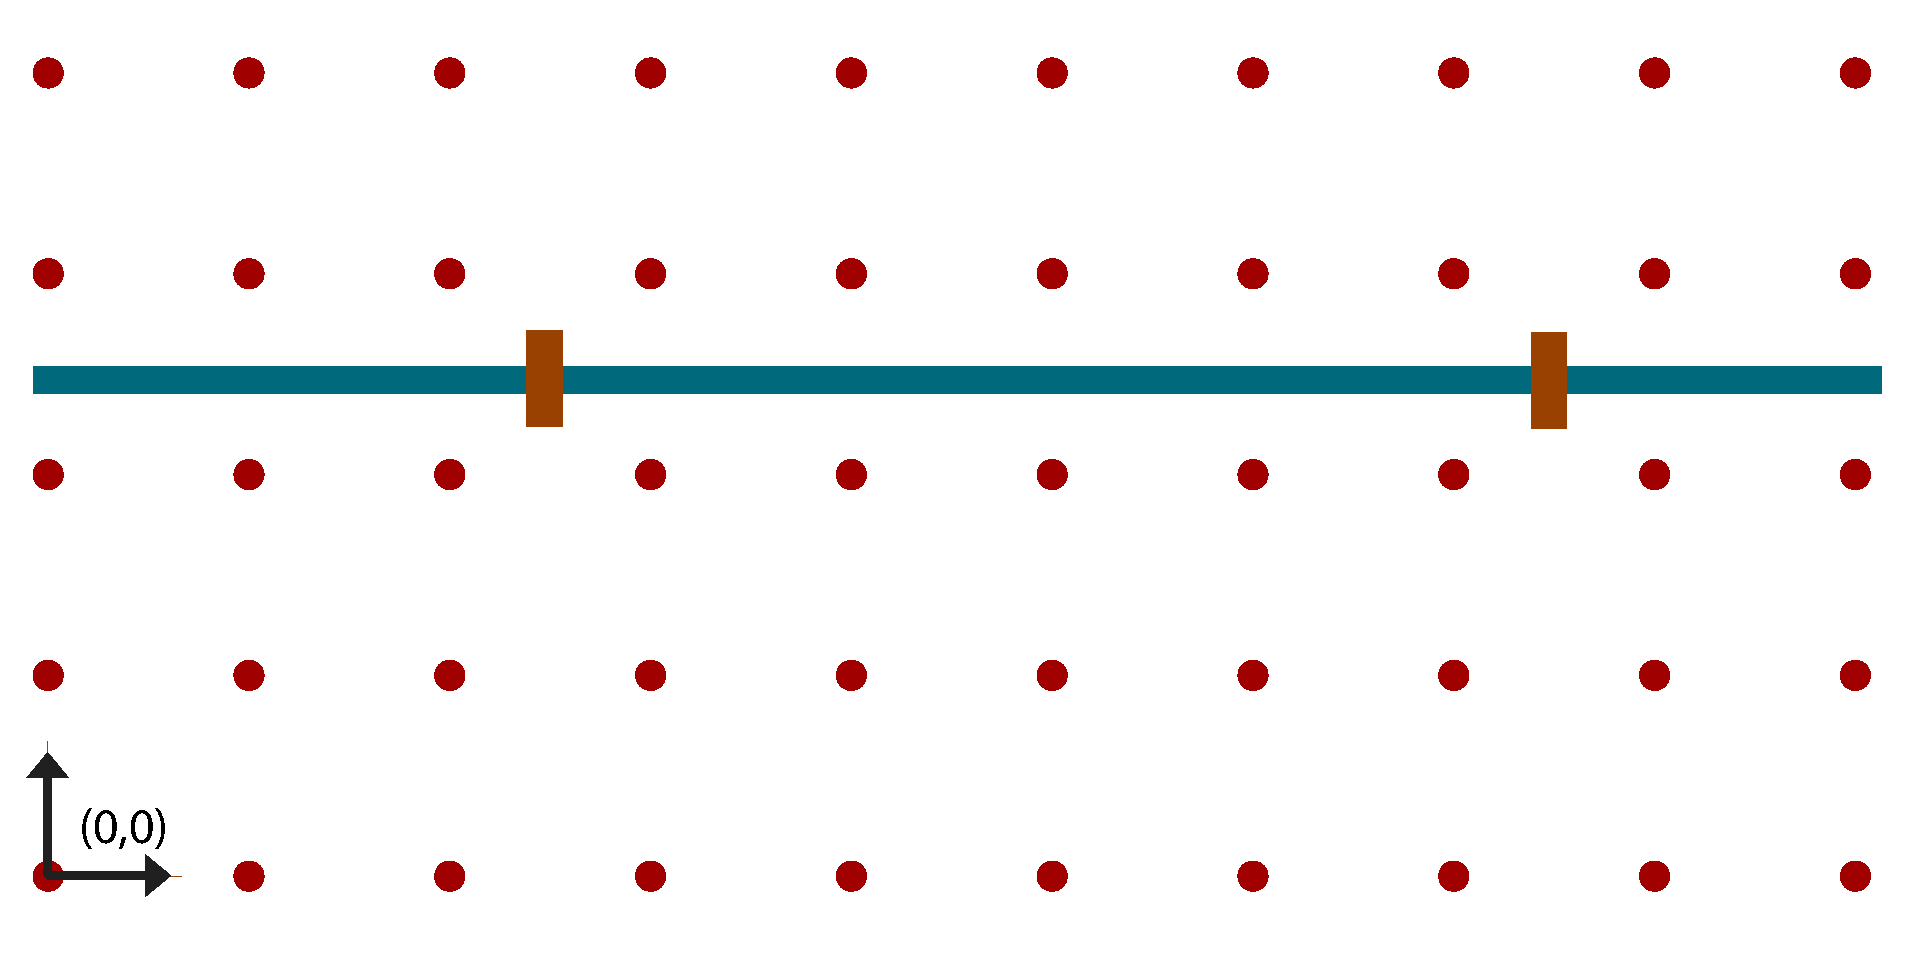
\includegraphics[width=0.8\linewidth]{images/diagram.pdf}
\caption{Diagram showing the layout of the town}
\label{fig:diagram}
\end{figure}

\bigskip

\noindent This report described two approaches to solve this Optimization problem. The first one uses a Genetic Algorithm, the second one uses Particle Swarm Optimization. These solutions to the given problem are described in the following sections. In the Appendix, the output of the program is shown. The general Objective function is described in the section below.

\section{Formulation of objective function}
\subsection{Explanation}
\noindent Multiple choices where considered for the implementation of the objective function for this problem. One possible solution for the objective function could have been the \textbf{Manhattan distance}\footnote{http://en.wikipedia.org/wiki/Taxicab\_geometry} between the possible location of the Fire Station and all the buildings in the city. 

\bigskip

\noindent Instead, Since there is no information is available about roads and the size of the buildings, the \textbf{Euclidian distance} between the possible locations for the buildings was chosen instead. Some modification is required because of the river running through the town: When the cost between two locations on the same side of the river is calculated, the normal Euclidian distance is used: 
\[
P_1 = (x_1, y_1), \quad P_2 = (x_2, y_2)
\]
\[
d(P_1, P_2) = \sqrt{(x_2 - x_1)^2 + (y_2 - y_1 )^2 }
\]
When the two locations are on opposing sides of the river. The Euclidian distances between the first location and the two bridges and between the two bridges and the second location are calculated. The minimum of these two distance is chosen as the cost between the two locations. $B_1, B_2$ are the locations of the two bridges.

\[
d(P_1, P_2) = \text{min} \; \left\{
\begin{array}{l}
d(P_1, B_1) + d(B_1, P_2 )\\
d(P_1, B_2) + d(B_2, P_2 )
\end{array} \right.
\]

\noindent The total cost of a possible location $Q$ for the fire station is the sum of the distances between the possible location and all the other locations.
\[
\text{cost}(Q) = \sum_{P \in \text{locations}} d(P,Q)
\]

\noindent The implementation of this objective function can be seen in section \ref{sec:matlab1}

\subsection{Objective function graph}
In Figure \ref{fig:plots}, the objective function is plotted for all possible locations of the fire station inside the town. It is obvious from the mesh and contourplot that there is a local maximum around the line of the river $j = 3.5$. The code to generate this graph is listed in section \ref{sec:matlab1}.
\begin{figure}[H]
\centering
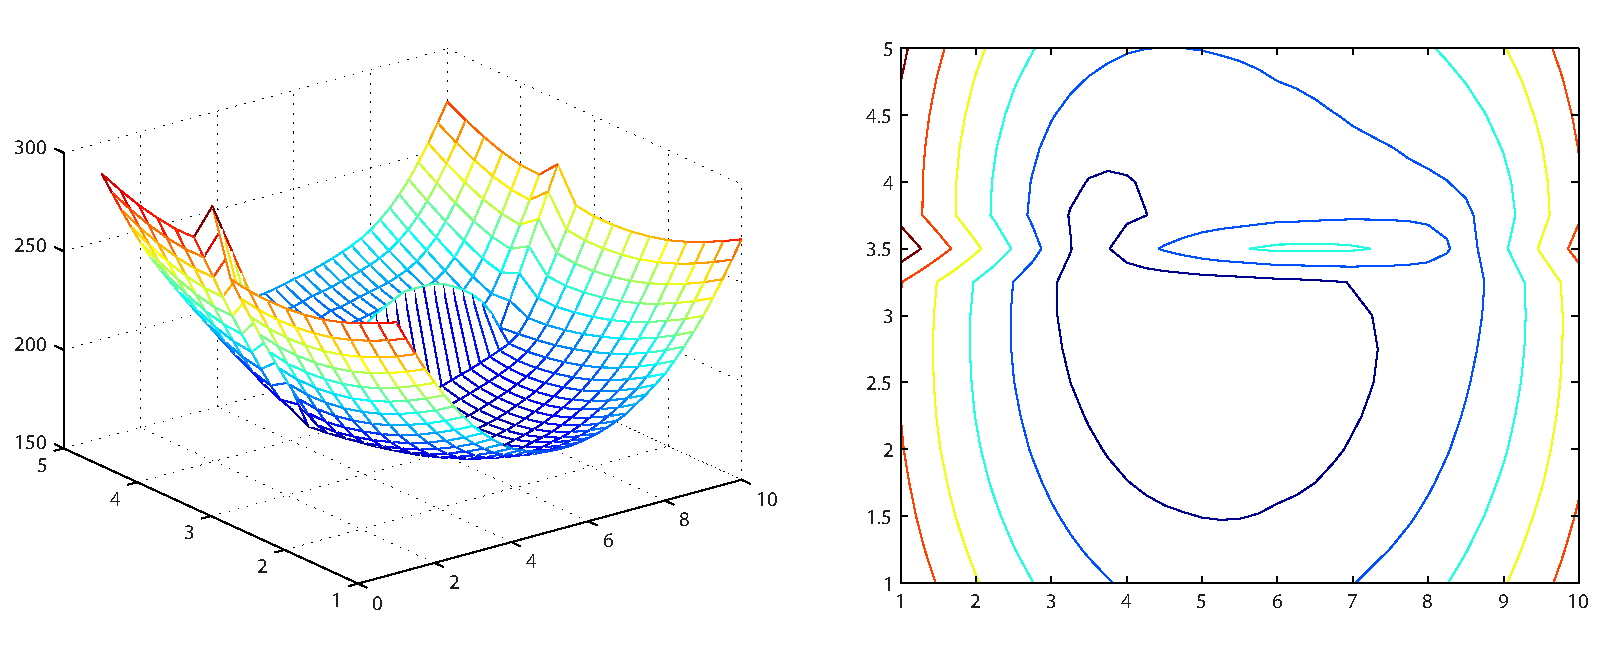
\includegraphics[width=0.95\linewidth]{images/plots.pdf}
\caption{A mesh and a contourplot showing the objective function.}
\label{fig:plots}
\end{figure}

\subsection{Matlab code}
\label{sec:matlab1}

\noindent The following code is used to calculated all the possible locations inside the town
\lstinputlisting[caption= Function to calculate  all the possible locations]{Matlab/calculateGrid.m}

\newpage

\noindent The following code is used to calculate the distance between two locations.
\lstinputlisting[caption= Function to calculate the distance between two points]{Matlab/euclidianDistance.m}

\noindent The following code calculates the total cost of a given position to all the other positions in the town.

\lstinputlisting[caption= Function to calculate the cost of a particular point in the town]{Matlab/cost.m}

\newpage

\noindent The following script was used to generate the plots shown in Figure \ref{fig:plots}.
\lstinputlisting[caption= Script to generate the plots]{Matlab/plotCost.m}

\section{Specification of search space}
The search space is a collection of discrete points given by:
\[
	(i,j) \quad i= i = 1,2,\cdots, 10 \quad  \text{and} j = 1,2, \cdots, 5
\]
\section{Genetic Algorithm}
\subsection{Explanation}
Since the search space is defined by a collection of discrete points, a two dimensional point is chosen as a chromosome in this genetic algorithm. The genes are the coordinates of the points. The algorithm described in section \ref{sec:matlab2} functions as follows.

\begin{enumerate}
\item An initial population with \texttt{n} chromosomes is generated by generating random discrete points within the town. with $ 1 \leq i \leq 10$ and $ 1 \leq j \leq 5$.
\item The  algorithm sorts the  population.
\item the \texttt{nS} best results are selected as possible parents for the next generation.
\item \texttt{ChildSize} Children are generated via crossover by selecting two parents with a random exponential system.
\item There is a change \texttt{mut} that mutation occurs in the genes of the child.
\item the children are stored for the next generation.
\item The possible parents are also kept for the next generation.
\item Some of the remaining chromosomes are selected to fill the rest of the generation. These are the \texttt{Survivors}.
\item Random mutations can occur in the \texttt{Survivors} with a change of \texttt{mut}.
\item This process repeats itself for \texttt{it} iterations.
\end{enumerate}

\subsection{Matlab code}
\lstinputlisting[caption= The function for the genetic algorithm]{Matlab/geneticAlgorithm.m}

\subsection{Parameters, Population Size and Convergence}
After several executions of the genetic algorithm, the following parameters seemed well suited to find a solution quickly.

\paragraph{Population Size = 10} A population size of ten seemed to fit the purpose of the algorithm well. (\texttt{PopulationSize} in the genetic algorithm in the code).
\paragraph{Parent Size = 3} The number of possible parents to be selected and stored for the next generation.
\paragraph{Child Size = 3} The number of children generated by the possible parents.
\paragraph{Number of Survivors} is equal to the population size minus the children an the parents.
\paragraph{Mutation Chance = 0.1} The change that a gene mutates on the transition of one generation to the next.
\paragraph{iterations = 15} The number of generations that needs to be generated before the algorithm stops executing.

\bigskip

\noindent These parameters caused convergence to appear rapidly. The Optimum often appeared in early generations. Almost the entire population is always converged to the optimum at the end of 15 iterations.

\medskip

\noindent \textbf{The output of this algorithm can be found in appendix \ref{sec:genMatlab}}
\section{Particle Swarm Optimization}
\appendix
\section{Genetic Algorithm: Matlab output}
\label{sec:genMatlab}
\lstinputlisting[captionpos=t, flexiblecolumns=true,frame=none, caption= The output from matlab for the genetic algorithm]{output1.txt}
\section{Particle Swarm Optimization: Matlab Output}
\end{document}